\documentclass{article}

\usepackage{graphicx}
\usepackage{tikz}
\usepackage{tikzsymbols}
\usetikzlibrary{calc,patterns,shapes.geometric}
\pagestyle{empty}
\usepackage[margin=0pt]{geometry}
\geometry{papersize={14in,12in}}

\def\centerarc[#1](#2)(#3:#4:#5){\draw[#1] ($(#2)+({#5*cos(#3)},{#5*sin(#3)})$) arc (#3:#4:#5);}

\begin{document}
	\begin{figure}
		\centering
		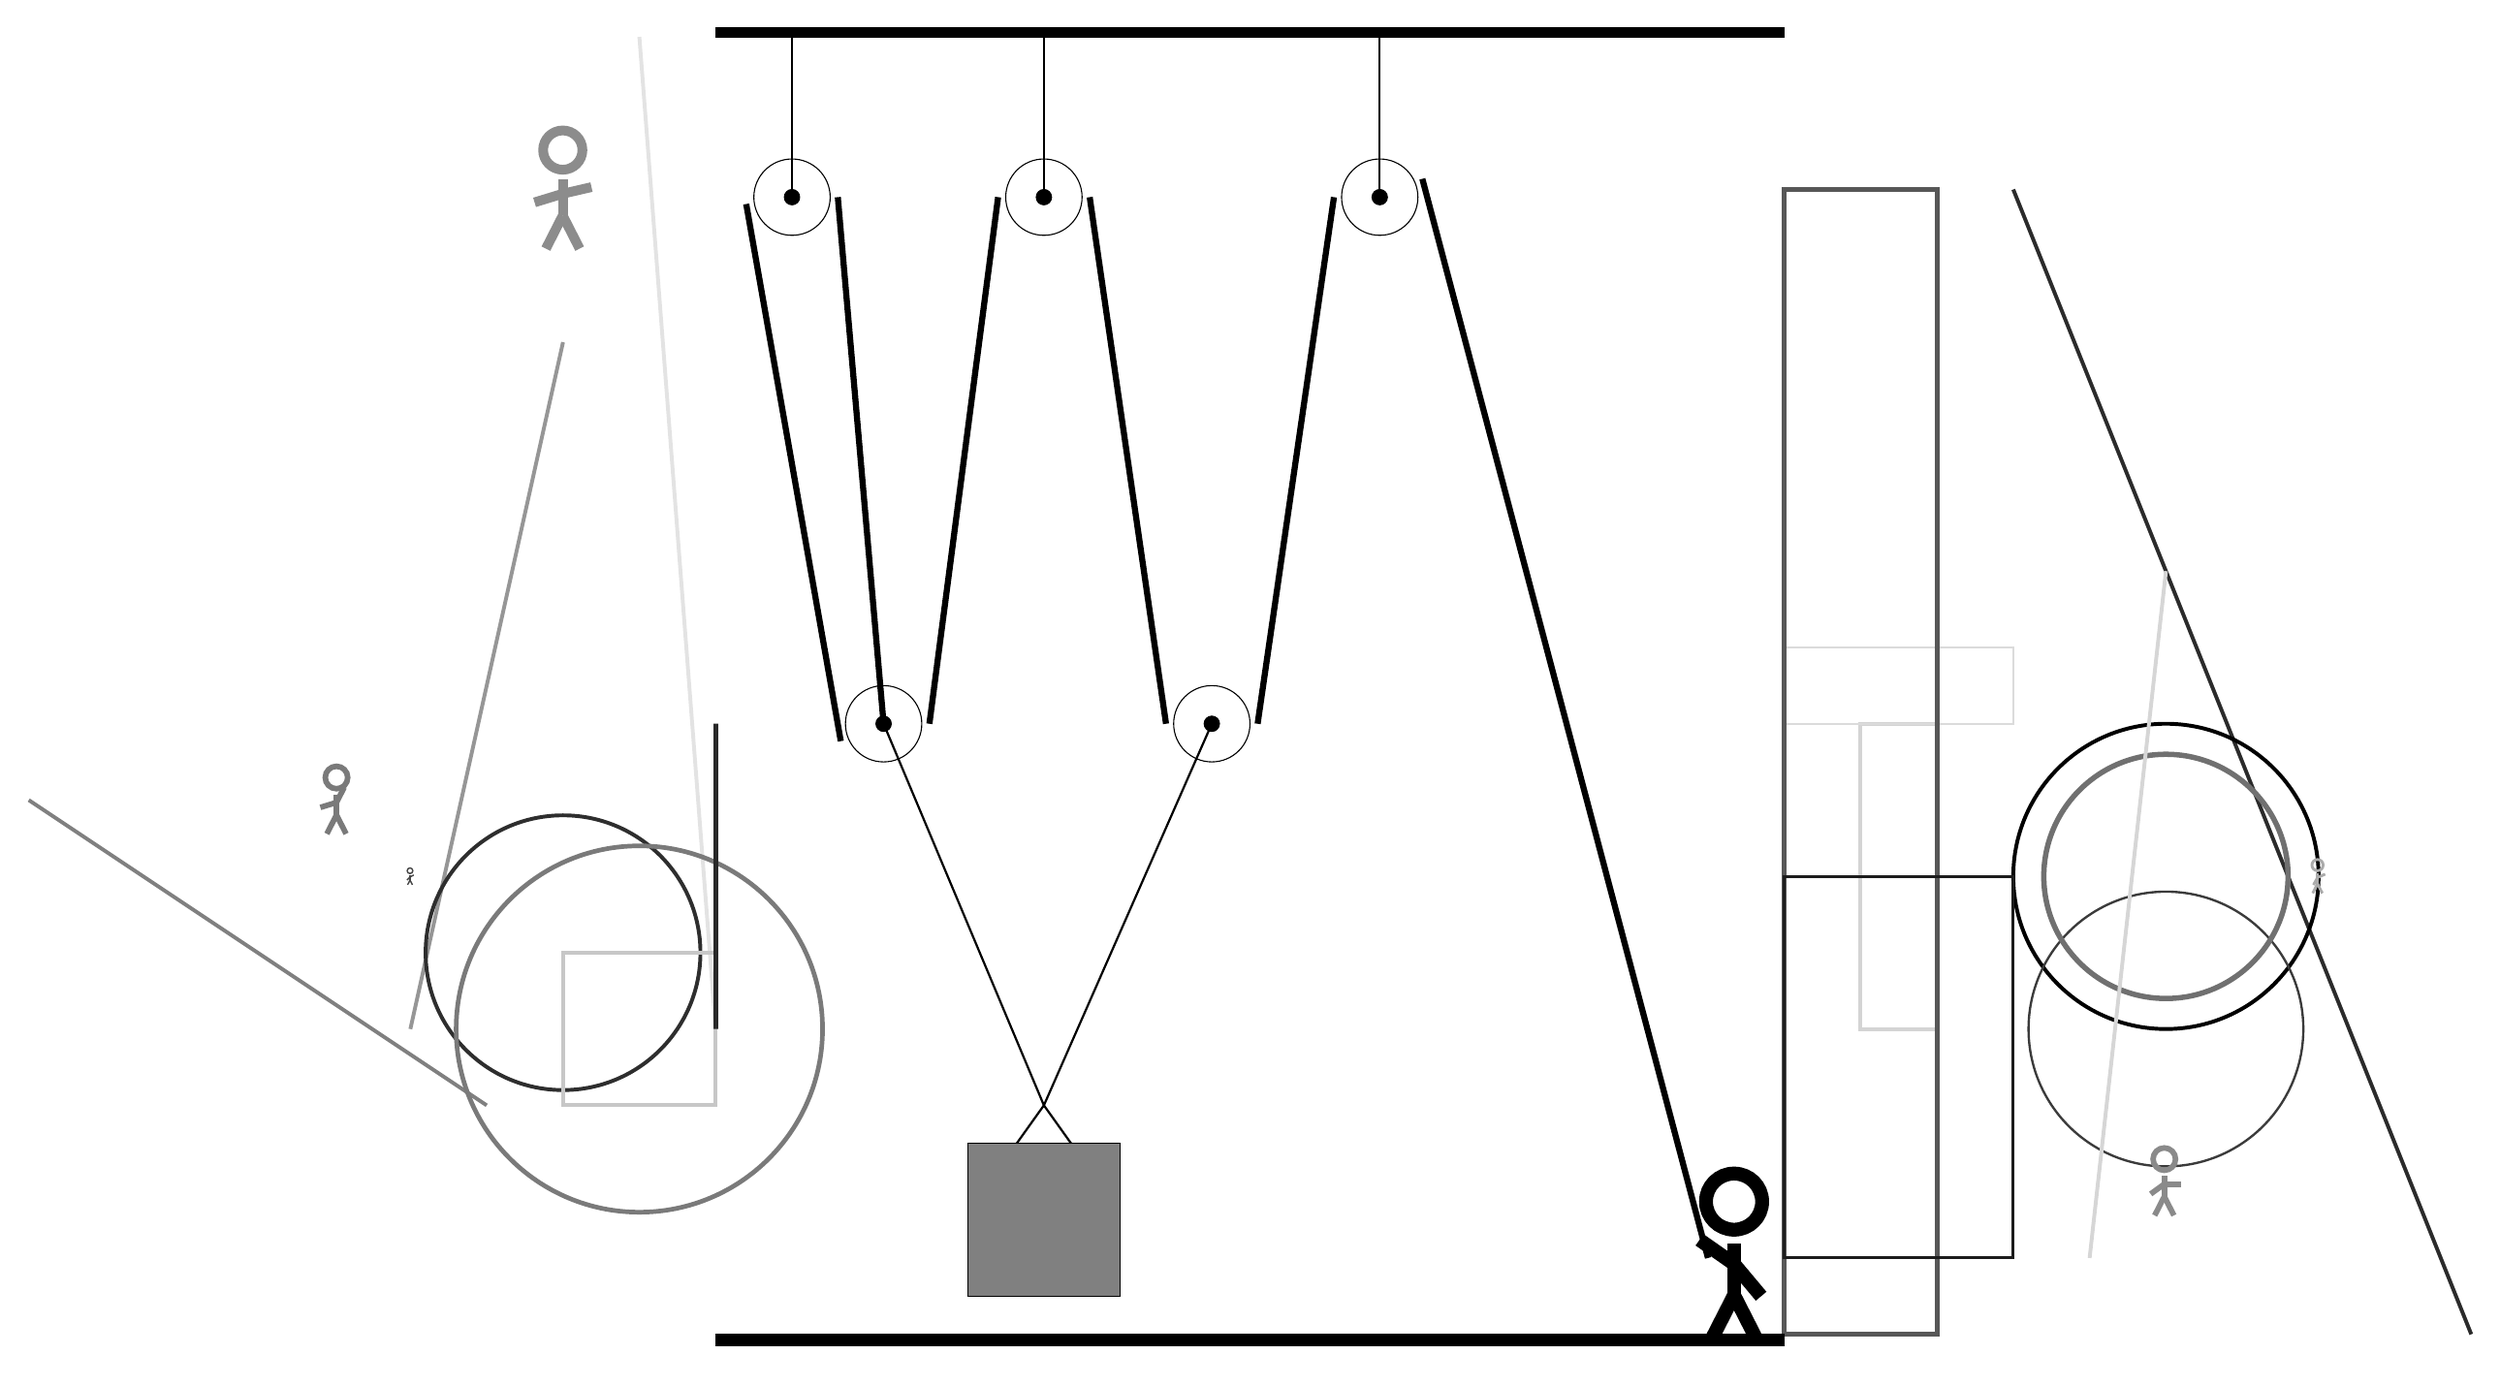
\begin{tikzpicture}
			%%%%% START %%%%%
			
			\draw[fill=black] (-2, 14) rectangle (12, 14.125);
			
			\draw (-1, 11.9) circle (0.5);
			\draw[fill=black] (-1, 11.9) circle (0.1);
			\draw[thick] (-1, 11.9) -- (-1, 14);
			
			\draw (2.3, 11.9) circle (0.5);
			\draw[fill=black] (2.3, 11.9) circle (0.1);
			\draw[thick] (2.3, 11.9) -- (2.3, 14);
			
			\draw (6.7, 11.9) circle (0.5);
			\draw[fill=black] (6.7, 11.9) circle (0.1);
			\draw[thick] (6.7, 11.9) -- (6.7, 14);
			
			\draw (0.2, 5) circle (0.5);
			\draw[fill=black] (0.2, 5) circle (0.1);
			
			\draw (4.5, 5) circle (0.5);
			\draw[fill=black] (4.5, 5) circle (0.1);
			
			\draw[thick] (0.2, 5) -- (2.3, 0)  -- (4.5, 5);
			\draw[thick]  (1.8, -0.7) -- (2.3, 0) -- (2.8, -0.7);
			\draw[fill=black!50] (1.3, -0.5) rectangle (3.3, -2.5);
			
			\draw[line width=0.8mm] (0.2, 5) -- (-0.4, 11.9);
			\centerarc[line width=0.8mm](-1, 11.9)(0:200:0.6);
			\draw[line width=0.8mm] (-1.6, 11.81) -- (-0.361, 4.772);
			\centerarc[line width=0.8mm](0.2, 5)(200:360:0.6);
			\draw[line width=0.8mm](0.8, 5) -- (1.7, 11.9);
			\centerarc[line width=0.8mm](2.3, 11.9)(0:180:0.6);
			\draw[line width=0.8mm] (2.9, 11.9) -- (3.9, 5);
			\centerarc[line width=0.8mm](4.5, 5)(180:360:0.6);
			\draw[line width=0.8mm] (5.1, 5) -- (6.1, 11.9);
			\centerarc[line width=0.8mm](6.7, 11.9)(20:180:0.6);
			\draw[line width=0.8mm](7.258, 12.14)  -- (11, -2);
			
			\draw[line width=0.5mm, color=black!17] (13, 1) rectangle (14, 5);
			
			\draw[line width=0.5mm, color=black!83](15, 12) -- (21, -3);
			\node[line width=0.5mm, color=black!45] at (-4, 12) {\Strichmaxerl[7][17][13]};
			\draw [line width=0.5mm, color=black!100](17, 3) circle (2.0);
			\draw[line width=0.5mm, color=black!50](-5, 0) -- (-11, 4);
			\draw[line width=0.5mm, color=black!41](-4, 10) -- (-6, 1);
			\draw[line width=0.2mm, color=black!14] (12, 5) rectangle (15, 6);
			
			\node[line width=0.3mm, color=black!33] at (19, 3) {\Strichmaxerl[2][61][24]};
			\draw [line width=0.5mm, color=black!82](-4, 2) circle (1.8);
			\node[line width=0.5mm, color=black!52] at (-7, 4) {\Strichmaxerl[4][17][63]};
			
			\draw[line width=0.5mm, color=black!11](-3, 14) -- (-2, 1);
			\draw [line width=0.6mm, color=black!52](-3, 1) circle (2.4);
			\draw [line width=0.3mm, color=black!77](17, 1) circle (1.8);
			
			\draw[line width=0.6mm, color=black!66] (12, 12) rectangle (14, -3);
			\node[line width=0.7mm, color=black!46] at (17, -1) {\Strichmaxerl[4][36][0]};
			\draw [line width=0.7mm, color=black!56](17, 3) circle (1.6);
			\node[line width=0.6mm, color=black!72] at (-6, 3) {\Strichmaxerl[1][45][28]};
			\draw[line width=0.4mm, color=black!89] (12, 3) rectangle (15, -2);
			\draw[line width=0.5mm, color=black!22] (-2, 2) rectangle (-4, 0);
			\draw[line width=0.7mm, color=black!84] (-2, 5) rectangle (-2, 1);
			\draw[line width=0.5mm, color=black!16](16, -2) -- (17, 7);
			
			\node at (11.3, -2) {\Strichmaxerl[10][-35][-50]};
			
			\draw[fill=black] (-2, -3) rectangle (12, -3.15);
			
			%%%%% END %%%%%
		\end{tikzpicture}
	\end{figure}	
\end{document}